\documentclass[12pt]{article}


\usepackage{amssymb}
\usepackage{amsmath}
\usepackage{fullpage}
\usepackage{epsfig}
\usepackage{epstopdf, xcolor, hyperref}
\everymath{\displaystyle}
\usepackage{enumerate}



\begin{document}

\begin{center}
\underline{\LARGE{Rectangular Coordinates, Spheres, \& Cylindrical Surfaces}}
\end{center}

\noindent SUGGESTED REFERENCE MATERIAL:

\bigskip

\noindent As you work through the problems listed below, you should reference Chapter 11.1 of the recommended textbook (or the equivalent chapter in your alternative textbook/online resource) and your lecture notes.

\bigskip

\noindent EXPECTED SKILLS:

\begin{itemize}

\item Be able to determine the location of a point in space using rectangular coordinates.

\item Be able to find the distance between and the midpoint of two points in space.

\item Know the standard equation of a sphere and be able to find the center and radius of a sphere. 

\item Be able to sketch cylindrical surfaces.

\end{itemize}

\noindent PRACTICE PROBLEMS:

\medskip

\noindent {\bf Problems 1-3 refer to the rectangular box, shown below.  The base of the rectangular box is in the $xy$-plane.}

\begin{center}
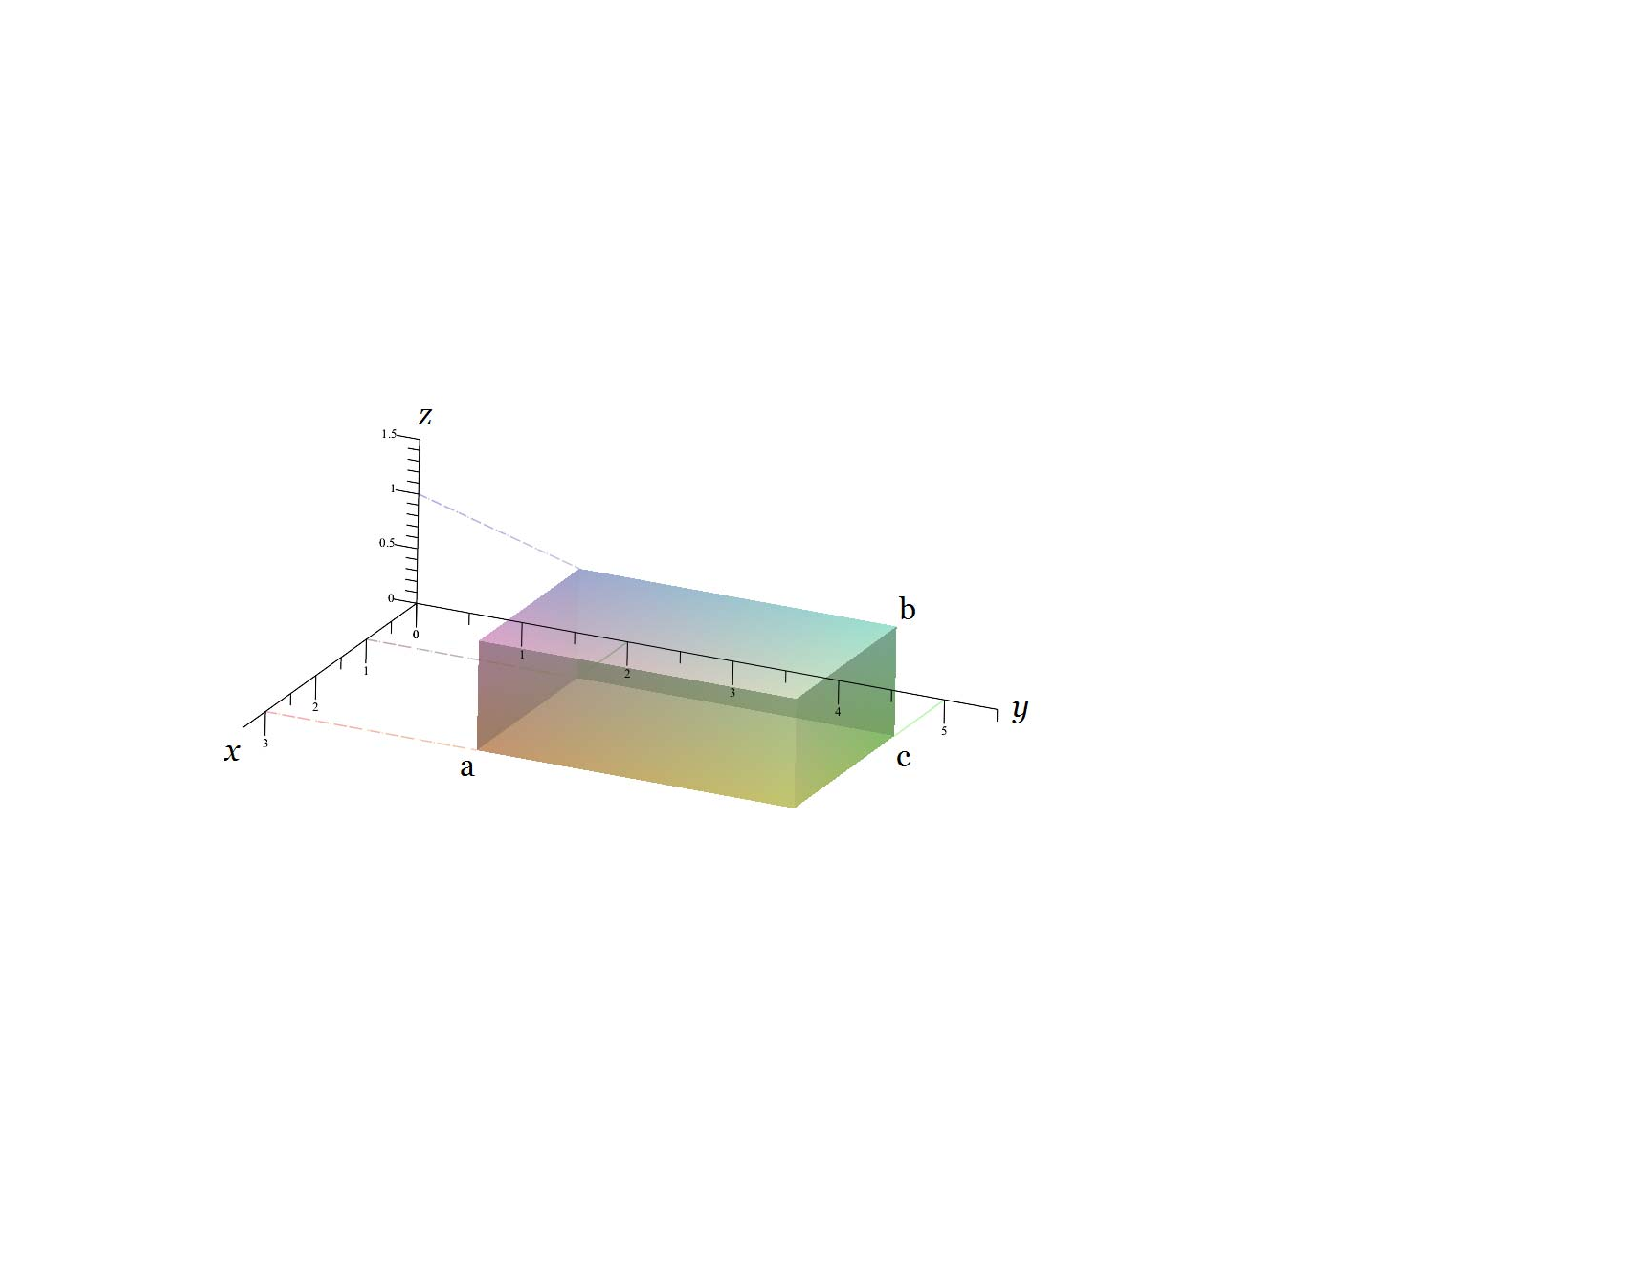
\includegraphics[scale=0.7]{box.pdf}
\end{center}

\begin{enumerate}

\item Find the coordinates of the eight corners of the box

\includegraphics[scale=0.5]{start.pdf}
{{$(1,2,0), (3,2,0), (3,5,0), (1,5,0), (1,2,1), (3,2,1), (3,5,1), (1,5,1)$}}
\includegraphics[scale=0.5]{end.pdf}


\item Compute the midpoint of the diagonal which extends from vertex $a$ to vertex $b$.

\includegraphics[scale=0.5]{start.pdf}
{{$\left(2,\frac{7}{2},\frac{1}{2}\right)$}}
\includegraphics[scale=0.5]{end.pdf}


\item Consider the triangle with vertices $a$, $b$, and $c$.

\begin{enumerate}

\item Compute the length of each of the three sides.

\includegraphics[scale=0.5]{start.pdf}
{{{0.8\linewidth}{The diagonal from vertex $a$ to vertex $b$ has length $\sqrt{14}$;\\
The line segment from vertex $a$ to vertex $c$ has length $\sqrt{13}$;\\
The line segment from vertex $c$ to vertex $b$ has length 1.}}}
\includegraphics[scale=0.5]{end.pdf}


\item Verify that the triangle is a right triangle.

\includegraphics[scale=0.5]{start.pdf}
{{{1\linewidth}{Notice that $\left(\sqrt{13}\right)^2+1^2=\left(\sqrt{14}\right)^2$.  So, the sides of the triangle (which are not collinear) satisfy the Pythagorean Theorem.  Thus, the triangle is a right triangle.}}}
\includegraphics[scale=0.5]{end.pdf}


\item Compute the angle between the diagonal which extends from vertex $a$ to vertex $b$ and the line segment which extends from vertex $a$ to vertex $c$.

\includegraphics[scale=0.5]{start.pdf}
{{$\cos^{-1}\left(\frac{\sqrt{13}}{\sqrt{14}}\right)$}}
\includegraphics[scale=0.5]{end.pdf}


\end{enumerate}

\item Consider the triangle with vertices $A(5,-2,-1)$, $B(7,0,3)$, and $C(9,-4,1)$.

\begin{enumerate}

\item Show that the triangle is an equilateral triangle.

\includegraphics[scale=0.5]{start.pdf}
{{The length of all sides of the triangle is $\sqrt{24}$; Detailed Solution: \textcolor{blue}{\href{http://www.math.drexel.edu/classes/Calculus/resources/Math200HW/Solutions/01_200_Rectangular_04.pdf}{Here}}}}
\includegraphics[scale=0.5]{end.pdf}


\item Compute the area of the triangle.

\includegraphics[scale=0.5]{start.pdf}
{{$6\sqrt{3}$ square units; Detailed Solution: \textcolor{blue}{\href{http://www.math.drexel.edu/classes/Calculus/resources/Math200HW/Solutions/01_200_Rectangular_04.pdf}{Here}}}}
\includegraphics[scale=0.5]{end.pdf}


\end{enumerate}

\item Find an equation of the sphere whose center is $(3,0,2)$ and which has a diameter of 6.

\includegraphics[scale=0.5]{start.pdf}
{{$(x-3)^2+y^2+(z-2)^2=9$}}
\includegraphics[scale=0.5]{end.pdf}


\item Find an equation of the sphere whose center is $(4,2,-1)$ and which passes through the origin.

\includegraphics[scale=0.5]{start.pdf}
{{$(x-4)^2+(y-2)^2+(z+1)^2=21$}}
\includegraphics[scale=0.5]{end.pdf}


\item Find an equation of the sphere which contains points $A(1,3,2)$ and $B(4,3,7)$ and the distance between $A$ and $B$ is equal to the diameter of the sphere.

\includegraphics[scale=0.5]{start.pdf}
{{$\left(x-\frac{5}{2}\right)^2+(y-3)^2+\left(z-\frac{9}{2}\right)^2=\frac{17}{2}$; Video Solution: \textcolor{blue}{\href{https://www.youtube.com/watch?v=kX4rI7KYVa4}{Here}}}}
\includegraphics[scale=0.5]{end.pdf}


\item Does the origin lie inside of the sphere $(x-1)^2+(y+2)^2+(z+3)^2=13$?  Justify your answer.

\includegraphics[scale=0.5]{start.pdf}
{{{1\linewidth}{No.  The distance from the origin to the center $(1,-2,-3)$ is $\sqrt{14}$ which is greater than the radius, $\sqrt{13}$.}}}
\includegraphics[scale=0.5]{end.pdf}


\newpage

\item Consider the cube with a center at the origin which has sides of length 2 that are parallel to the coordinate planes.  

\begin{enumerate}

\item Compute an equation of the sphere which is inscribed in this cube.

\includegraphics[scale=0.5]{start.pdf}
{{$x^2+y^2+z^2=1$; Detailed Solution: \textcolor{blue}{\href{http://www.math.drexel.edu/classes/Calculus/resources/Math200HW/Solutions/01_200_Rectangular_09.pdf}{Here}}}}
\includegraphics[scale=0.5]{end.pdf}


\item Compute an equation of the sphere which is circumscribed around the cube.

\includegraphics[scale=0.5]{start.pdf}
{{$x^2+y^2+z^2=3$; Detailed Solution: \textcolor{blue}{\href{http://www.math.drexel.edu/classes/Calculus/resources/Math200HW/Solutions/01_200_Rectangular_09.pdf}{Here}}}}
\includegraphics[scale=0.5]{end.pdf}


\end{enumerate}

\item Find equations of the tangent spheres of equal radii whose centers are $(2,3,1)$ and $(5,-3,2)$, respectively.

\includegraphics[scale=0.5]{start.pdf}
{{$(x-2)^2+(y-3)^2+(z-1)^2=\frac{23}{2}$ and $(x-5)^2+(y+3)^2+(z-2)^2=\frac{23}{2}$}}
\includegraphics[scale=0.5]{end.pdf}


\item Sketch the following surfaces in space.

\begin{enumerate}

\item $3x+4y=12$\\

\includegraphics[scale=0.5]{start.pdf}
{{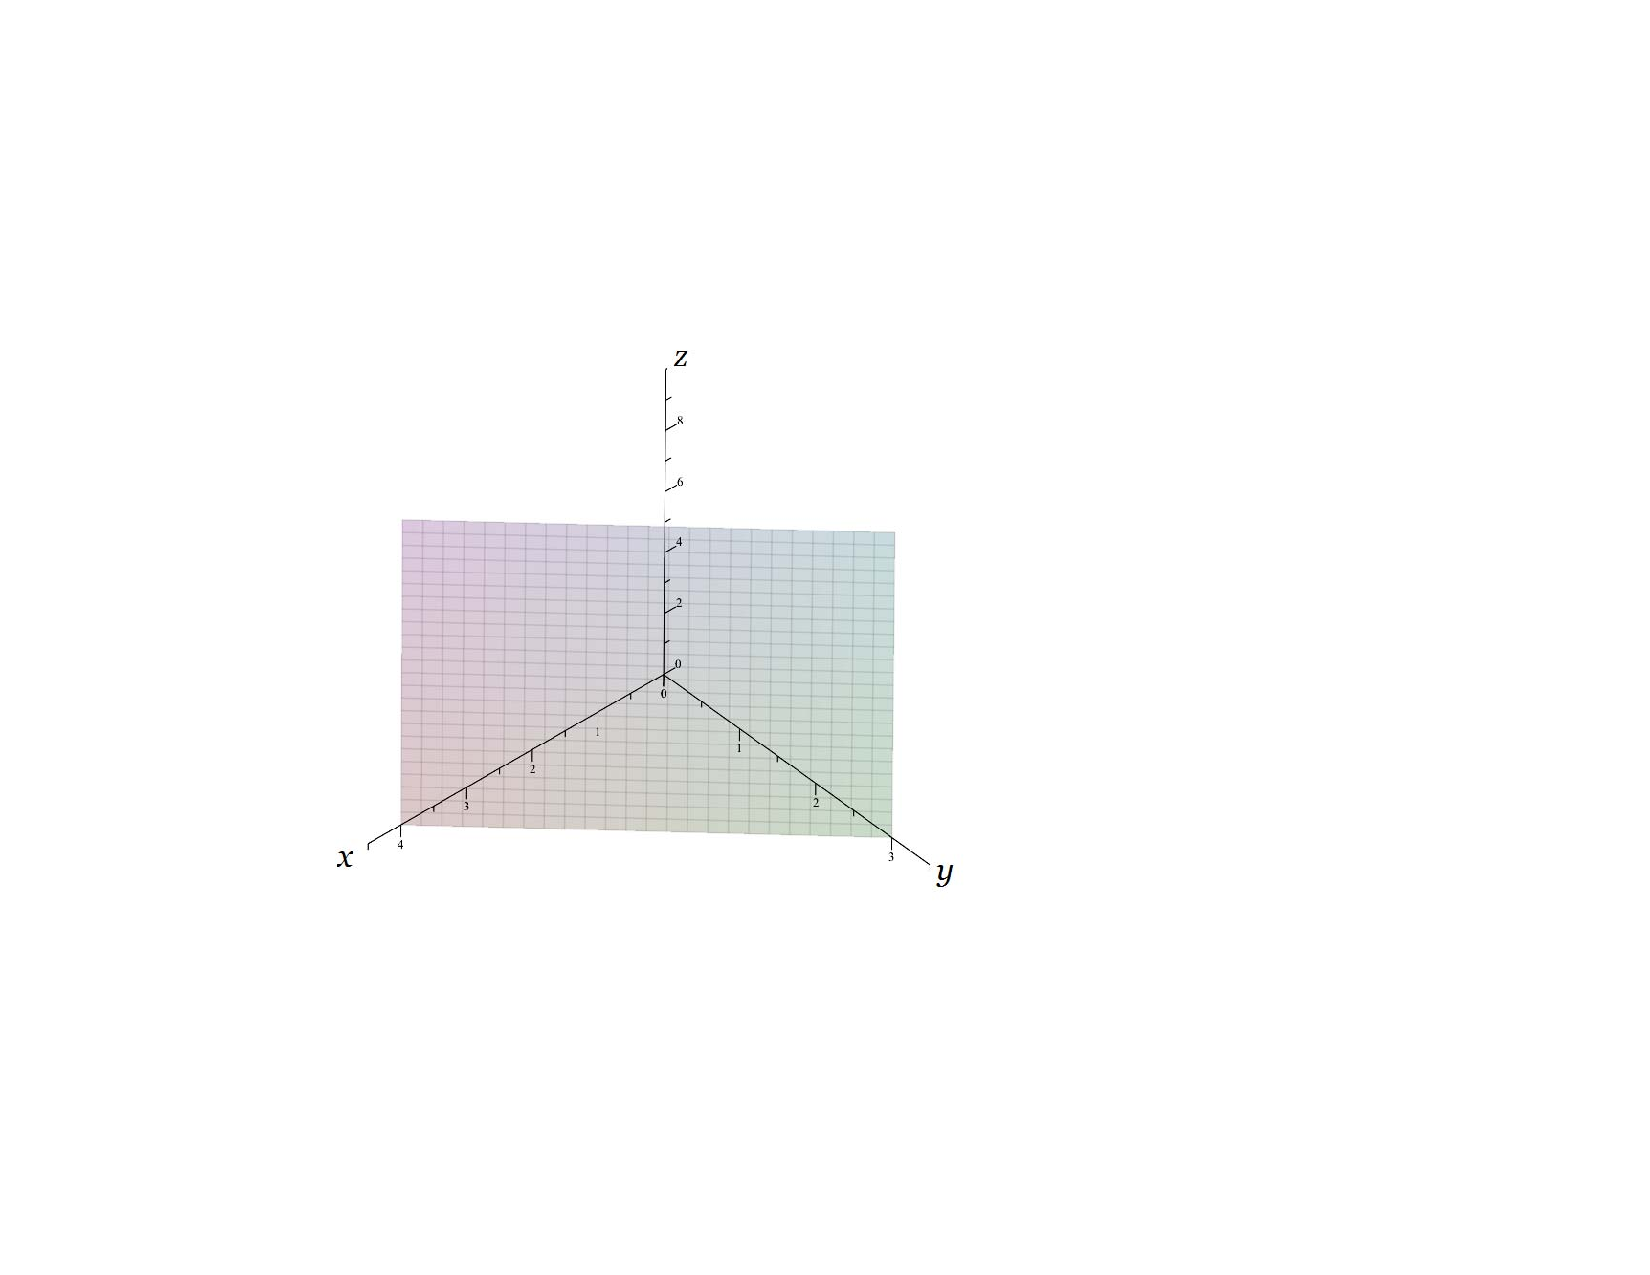
\includegraphics[scale=0.5]{plane.pdf}}}
\includegraphics[scale=0.5]{end.pdf}


\item $\frac{x^2}{4}+\frac{y^2}{9}=1$\\

\includegraphics[scale=0.5]{start.pdf}
{{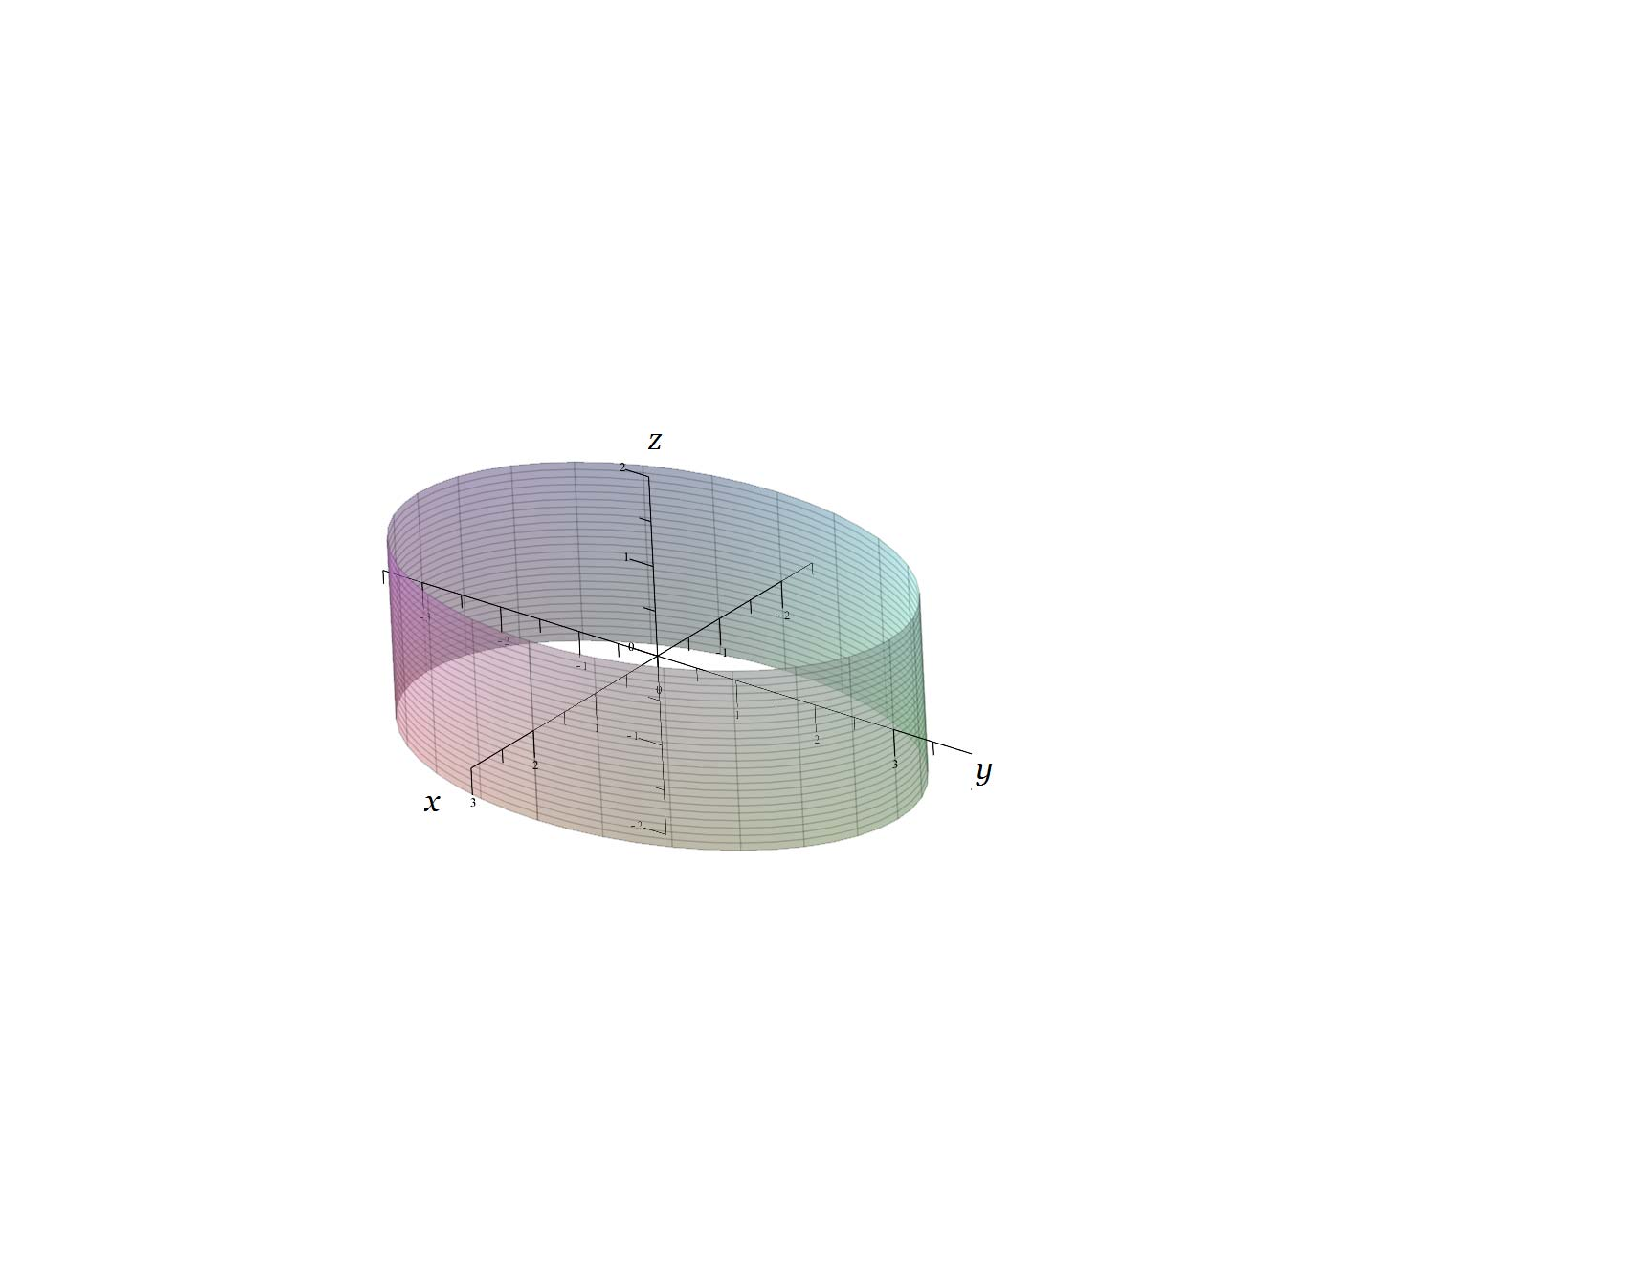
\includegraphics[scale=0.5]{ellipse.pdf}}}
\includegraphics[scale=0.5]{end.pdf}


\newpage

\item $z=x^2$\\

\includegraphics[scale=0.5]{start.pdf}
{{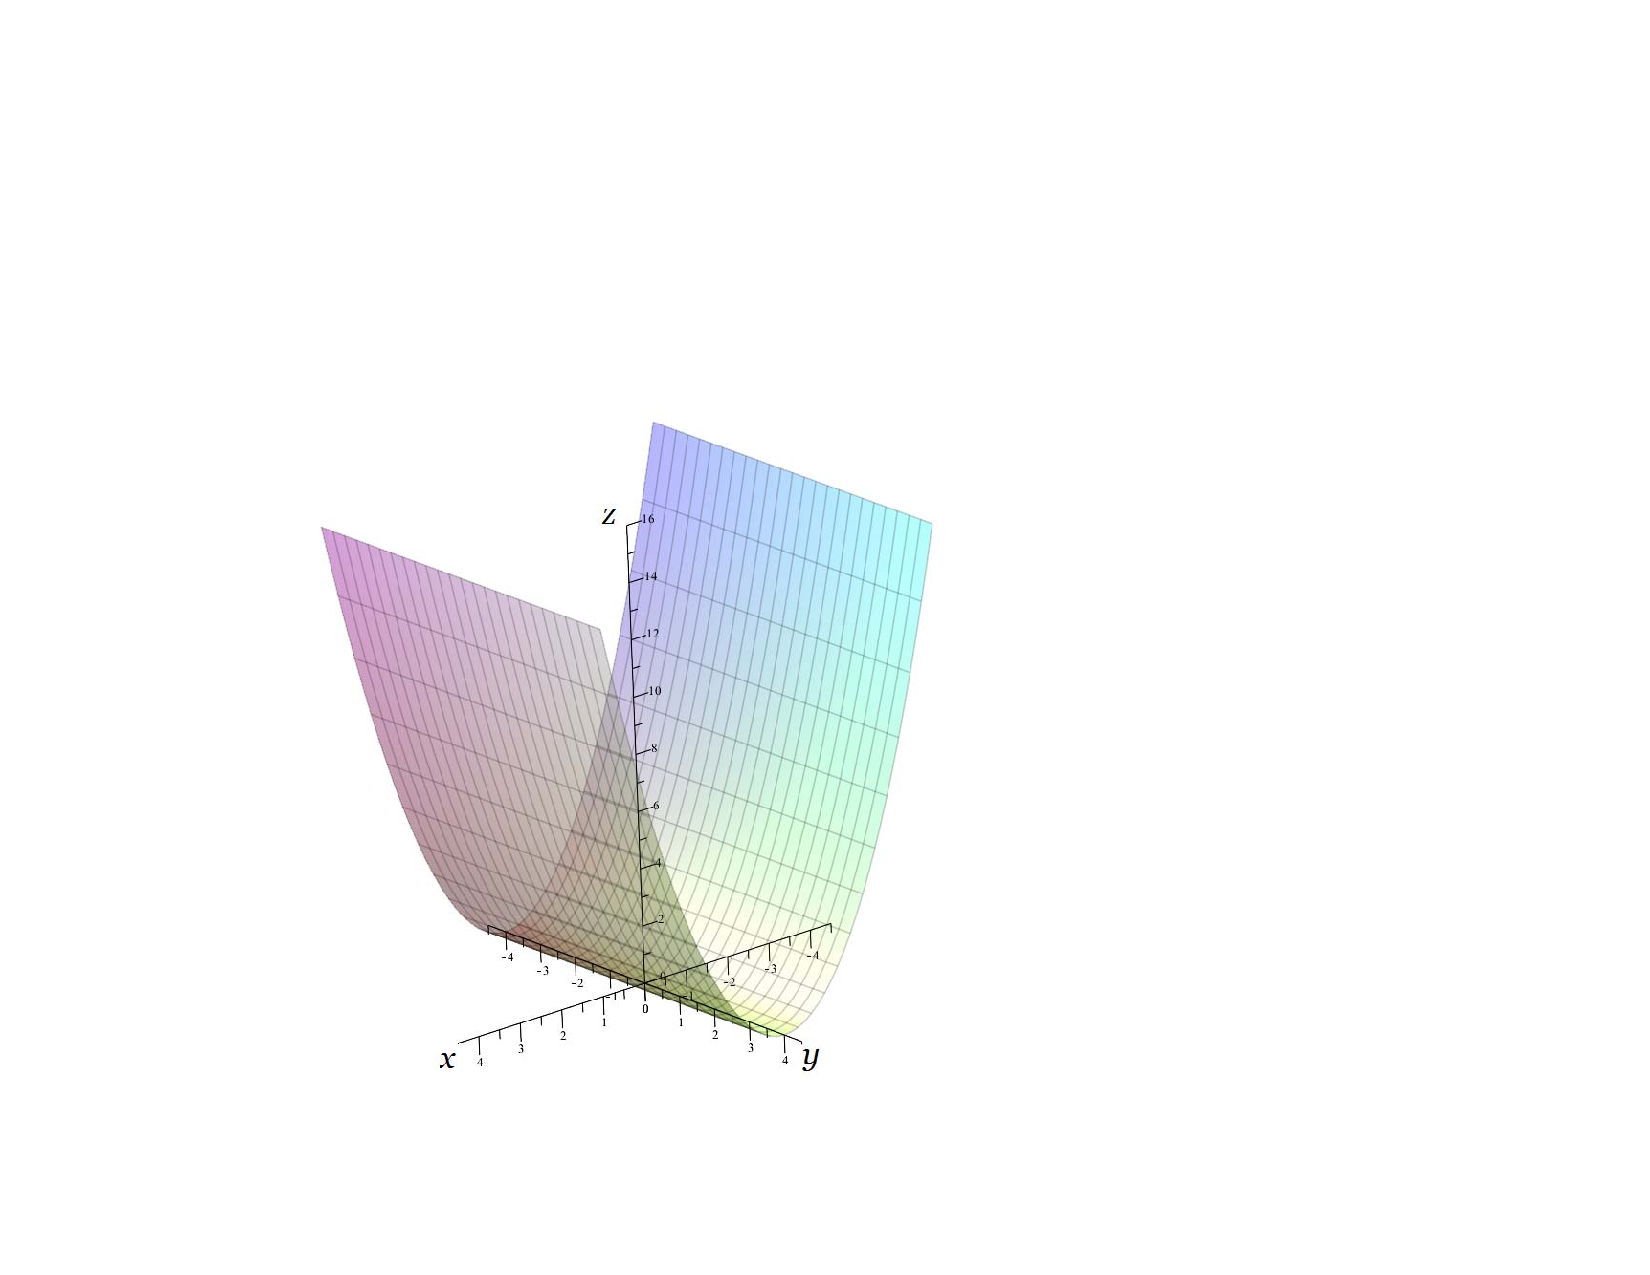
\includegraphics[scale=0.5]{parabola.pdf}}}
\includegraphics[scale=0.5]{end.pdf}


\item $z=e^y$

\includegraphics[scale=0.5]{start.pdf}
{{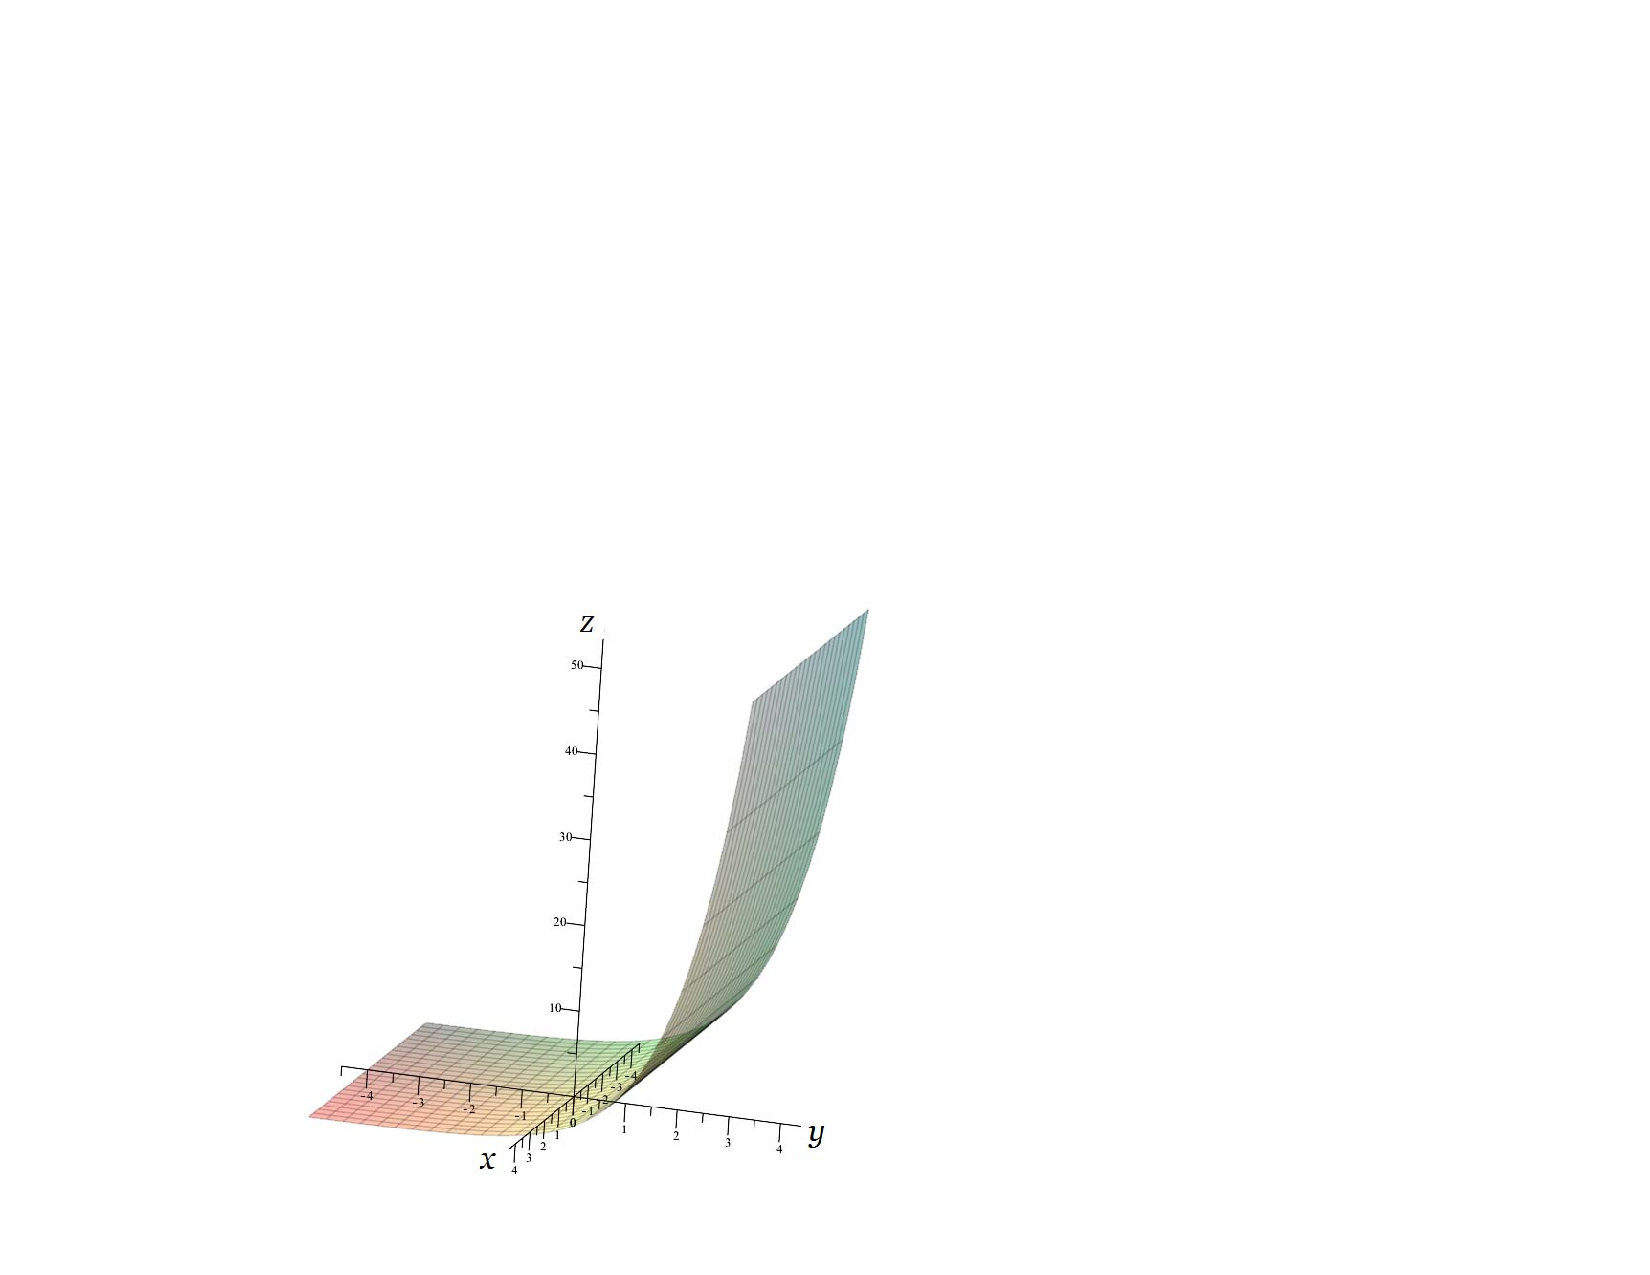
\includegraphics[scale=0.5]{expo.pdf}}}
\includegraphics[scale=0.5]{end.pdf}


\end{enumerate}

\item Describe all points in space whose coordinates satisfy the following inequality $$x^2+z^2-4x-8z+13>0$$

\includegraphics[scale=0.5]{start.pdf}
{{All points outside of the cylinder $(x-2)^2+(z-4)^2=7$; Detailed Solution: \textcolor{blue}{\href{http://www.math.drexel.edu/classes/Calculus/resources/Math200HW/Solutions/01_200_Rectangular_12.pdf}{Here}}}}
\includegraphics[scale=0.5]{end.pdf}


\item Consider the surface $x^2+y^2+z^2-4x-12y-8z=k$, where $k$ is a real number.  For which values of $k$ will the surface be a sphere?

\includegraphics[scale=0.5]{start.pdf}
{{$k>-56$}}
\includegraphics[scale=0.5]{end.pdf}


\end{enumerate}

\end{document}